\documentclass[11pt]{article}
\usepackage[review]{acl}
\usepackage{times}
\usepackage{latexsym}
\usepackage[T1]{fontenc}
\usepackage[utf8]{inputenc}
\usepackage{microtype}
\usepackage{inconsolata}
\usepackage{graphicx}
\usepackage{amsmath,amssymb,booktabs}
\hypersetup{pdfauthor={},pdftitle={When Does Knowledge Distillation Transfer? Controlled Evidence from Warm-Start Language Modeling}}

\title{When Does Knowledge Distillation Transfer? Controlled Evidence from Warm-Start Language Modeling}
\author{Anonymous authors}

\begin{document}
\maketitle
\begin{abstract}
Knowledge distillation (KD) is commonly evaluated by distilled-student performance, yet a basic question remains: given an already trained student, does teacher supervision improve over maximum-likelihood continuation from the same state? We study autoregressive language modeling through matched warm-start continuations, controlled teacher interventions, and independent student replications. Under the same token-normalized formulation, KD produces positive transfer on Penn Treebank and WikiText-2 and negative transfer on TinyStories, consistently across three student initializations per setting. We test several explanations. At fixed teacher architecture and fusion composition, changing the trained teacher state reverses transfer, showing that teacher state and predictive quality strongly modulate distillation. However, global teacher likelihood is insufficient: a teacher with worse held-out likelihood than the matched CE comparator still improves all three students. Greater branch disagreement and architectural heterogeneity do not imply better transfer; a homogeneous Transformer ensemble outperforms the heterogeneous Transformer--Grassmann teacher in all three comparisons. Tested local gradient and curvature diagnostics also fail to reliably predict long-horizon transfer. Together, these results support configuration-dependent distillability: whether KD helps depends on the teacher, warm-start student, and training configuration, rather than a single teacher-quality or compatibility statistic.
\end{abstract}

\section{Introduction}\label{sec:introduction}

Knowledge distillation (KD) transfers predictive information from a teacher to a smaller student. Autoregressive LM distillation now includes alternative divergences, on-policy training, adaptive supervision, and teacher selection. These developments make clear that stronger teachers do not automatically produce stronger students. A practical question precedes the choice of a more sophisticated algorithm: given a student that has already been trained, does frozen teacher supervision improve over continuing maximum-likelihood training from exactly the same state?

\begin{figure*}[!t]
\centering
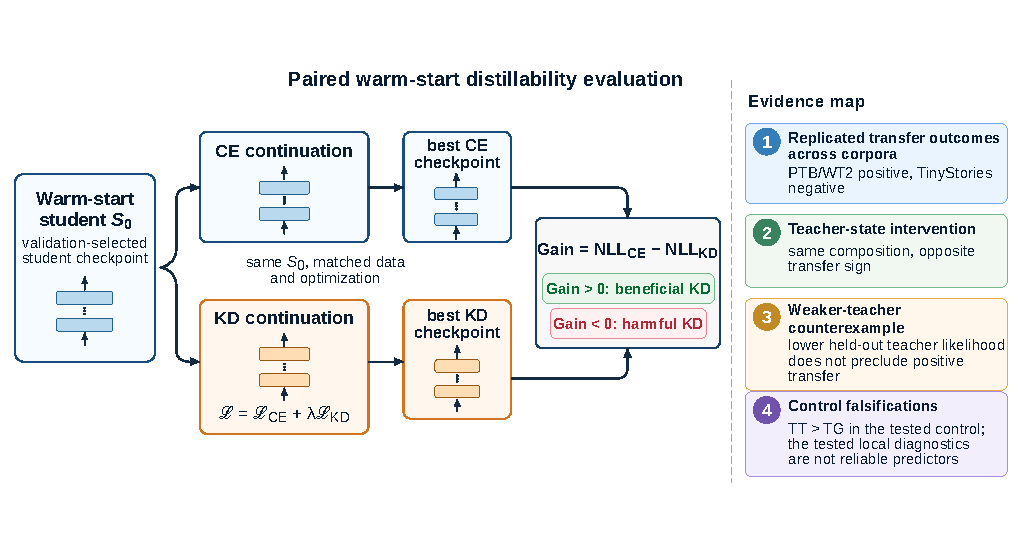
\includegraphics[width=\textwidth]{figures/fig1_paired_protocol.pdf}
\caption{Paired warm-start evaluation. Identical $S_0$ weights initialize CE and KD; independent validation selection precedes test reporting. The evidence map separates replicated transfer from bounded explanatory controls.}
\label{fig:paired_protocol}
\end{figure*}

We study this question through paired warm-start evaluation. A validation-selected student checkpoint $S_0$ initializes both a cross-entropy (CE) continuation and a KD continuation. Both arms use fresh optimizers and matched continuation data and budgets, then independently select checkpoints by validation likelihood. Their test-NLL difference measures the value of adding supervision beyond CE, not improvement over an unrelated baseline. Each confirmatory comparison uses three independently trained student initializations.

This design reveals reproducible positive and negative transfer under the same token-normalized KD formulation. Mean gains are $0.1449$ NLL on PTB and $0.1557$ on WikiText-2, whereas TinyStories degrades by $0.1072$. Every domain has the same direction across all three students. These results do not establish a causal effect of corpus identity: teachers, data amounts, and preparation histories differ. We therefore test candidate explanations with more controlled comparisons.

Teacher quality is an important but incomplete explanation. At fixed WikiText-2 teacher architecture, source identities, and fusion composition, a jointly trained teacher helps all three students, while a fusion-weight-only state harms all three. The paired contrast is $0.1833$ NLL. Teacher training state and resulting predictive quality strongly modulate transfer, but this intervention does not isolate scalar likelihood as the cause. Conversely, a Grassmann-only source with worse held-out likelihood than every matched validation-selected CE comparator still improves all three students. Global teacher likelihood alone therefore cannot determine distillability.

Within a fixed Transformer--Grassmann checkpoint, fused supervision transfers better than either component. A homogeneous Transformer--Transformer control nevertheless yields better KD endpoints in all three students, despite lower branch disagreement. Differences in teacher quality, parameter count, and training history prevent attributing this ordering to architecture. The control does not support uniquely transferable Grassmann representations or heterogeneous-supervision superiority.

Retrospective local gradient and curvature scores also misclassify several configurations with reproducibly positive endpoints. We treat these failures as bounded falsification evidence, not a new predictor or a universal impossibility result. The tested statistics do not summarize the long optimization trajectory and validation selection.

The contribution is a controlled empirical evidence chain: paired CE-relative positive and negative transfer, a fixed-composition teacher-state reversal, a weaker-source counterexample, a homogeneous-ensemble falsification, and failed retrospective local diagnostics. We do not propose a new KD algorithm or claim the first instance of harmful or weak-teacher KD. The practical implication is to assess teacher supervision against matched continuation from the student state of interest, rather than infer its value from a single teacher-quality, diversity, or local-compatibility statistic.

\section{Related Work}\label{sec:related-work}

\subsection{Teacher quality and student-oriented supervision}
KD transfers predictive distributions rather than only hard labels~\citep{hinton2015distilling}. Capacity mismatch and harmful late-training supervision already show that teacher quality and teaching utility differ~\citep{cho2019efficacy}; student-friendly teachers address this mismatch through student branches~\citep{park2021friendly}. Statistical analyses emphasize probability estimation and bias--variance trade-offs~\citep{menon2021statistical}, and poor classifiers can be useful teachers under specific assumptions~\citep{kaplun2022bad}. Our contribution is not the general observation that teacher accuracy can be insufficient, but the controlled warm-start LM evidence chain.

\subsection{Autoregressive LM distillation}
MiniLLM uses reverse KL and policy-gradient optimization~\citep{gu2024minillm}; GKD uses student-generated contexts and flexible divergences~\citep{agarwal2024gkd}. ATKD adapts supervision to easy and hard tokens~\citep{zhong2024atkd}, and selective NMT distillation identifies potentially harmful guidance~\citep{wang2021selective}. Distillation scaling laws relate student likelihood to teacher performance, size, and compute~\citep{busbridge2025scaling}. We instead hold corpus-based forward-KL continuation fixed and evaluate gain over CE from the same student. Our study does not compare generation quality or establish superiority over these methods.

\subsection{Adaptive, ensemble, and gradient-driven supervision}
Multi-teacher selection~\citep{yuan2021selection} and student quiz-set feedback in MetaDistil~\citep{zhou2022metadistil} address teacher suitability. Ensemble fidelity and generalization are distinct~\citep{stanton2021really}, while adaptive ensemble KD uses gradients to manage competing guidance~\citep{du2020agree}. AdaKD adapts token focus and temperature~\citep{xie2026adakd}; entropy-aware on-policy KD adds forward KL at uncertain tokens~\citep{jin2026entropy}. GRACE ranks teachers using spectral statistics of student gradients on teacher-generated responses~\citep{panigrahi2026grace}, unlike our fixed-logit validation-gradient probes. We do not evaluate these adaptive algorithms. Our controls and failed local diagnostics complement this literature without proposing a new compatibility theory.

\section{Paired Warm-Start Evaluation}\label{sec:problem-setting}

For each independently prepared student, a validation-selected $S_0$ initializes CE and CE+KD with identical weights and fresh optimizer states. Continuation data, order, optimizer, scheduler, and budget are matched. Each arm selects its checkpoint independently by validation NLL; test reporting follows selection (Figure~\ref{fig:paired_protocol}).

Let $p_{\mathrm{teach},i}^{(\tau)}$ and $p_{\mathrm{stud},i}^{(\tau)}$ denote next-token distributions at temperature $\tau$. Over valid target positions $\mathcal I$ after the causal shift, the objective is
\begin{align}
\mathcal L&=\mathcal L_{\mathrm{CE}}+\lambda\mathcal L_{\mathrm{distill}},\label{eq:kd-objective}\\
\mathcal L_{\mathrm{distill}}&=\frac{\tau^2}{|\mathcal I|}\sum_{i\in\mathcal I}
\mathrm{KL}\!\left(p_{\mathrm{teach},i}^{(\tau)}\|p_{\mathrm{stud},i}^{(\tau)}\right).\nonumber
\end{align}
Both losses average over target tokens. Primary KD fixes $\tau=2$ and $\lambda=5$; CE uses $\lambda=0$. The operational paired endpoint is
\begin{equation}
\mathrm{Gain}_{\mathrm{KD}}=\mathrm{NLL}_{\mathrm{CE}}^{\mathrm{test}}-\mathrm{NLL}_{\mathrm{KD}}^{\mathrm{test}}.
\label{eq:paired-gain}
\end{equation}
Positive gain favors KD over CE, not necessarily over $S_0$. This is a protocol-specific endpoint, not a theoretical measure of distillability.

We report seeds 42, 123, and 456, their mean paired gain, sample SD, and sign consistency. These vary student preparation, not teacher training or corpus sampling; SD is neither a standard error nor a significance test. Primary selection uses trained continuation checkpoints. A separately labeled diagnostic allows unmodified $S_0$ as step 0 without replacing the primary endpoints.

\section{Setting and Controlled Interventions}\label{sec:experimental-setting}

The primary corpora are PTB~\citep{marcus1993ptb}, WikiText-2~\citep{merity2016wikitext}, and TinyStories~\citep{eldan2023tinystories}. The 31.43M-parameter student uses a local GPT-2 tokenizer, sequence length 256, and 20-epoch preparation. Matched 10-epoch continuations use AdamW, learning rate $10^{-4}$, batch 32, weight decay 0.01, 5\% warmup with cosine decay, AMP, and clipping at 1. Teachers and preparation histories differ across corpora; absolute cross-domain NLL is not directly comparable. Appendices~\ref{app:architecture} and~\ref{app:protocols} give reproducibility details.

The heterogeneous test-bed teacher combines Transformer~\citep{vaswani2017attention} and causal Grassmann branches through late-logit fusion:
\begin{equation}
z_{\mathrm{TG}}=\alpha z^{(\mathrm T)}+(1-\alpha)z^{(\mathrm G)}.
\label{eq:teacher-fusion}
\end{equation}
The architecture is a supervision source, not a new method contribution. The WikiText-2 state intervention compares jointly trained J with fusion-weight-only A using identical source identities and deployed $\alpha=0.5$. The source ablation holds J fixed and uses $\alpha=0.5,1,0$ for fused (F/TG), Transformer-only (T), and Grassmann-only (G) supervision.

The homogeneous TT control adds an independently prepared Transformer with the same source architecture, data, tokenizer, and 20-epoch budget. TT then follows a 10-epoch joint teacher schedule with branches frozen in epoch 1; TT and TG both deploy $\alpha=0.5$. Their full training histories, fusion learning rates, parameter counts, and predictive quality are not identical.

Teacher-state and source likelihoods use the same 512-chunk validation subset (130,560 targets); TT/TG uses full validation. These scopes remain separate. WikiText-2 controls share CE and TG endpoints and are not additional independent replications. Retrospective local diagnostics and a pretrained SmolLM2/FineWeb-Edu stress test are reported separately from the primary matrix.

\section{Positive and Negative Transfer}\label{sec:cross-domain-transfer}

The same token-normalized formulation produces positive transfer on PTB and WikiText-2 and negative transfer on TinyStories (Table~\ref{tab:cross_domain_transfer}; Figure~\ref{fig:cross_domain_gain}). Every domain has identical gain direction across its three independent student preparations. On TinyStories, CE improves over $S_0$ in all three seeds, so harmful KD is relative to a useful continuation, not simply two unnecessary training arms.

These outcomes establish reproducibility for the tested configurations, not a causal corpus effect. Teachers, data amounts, and student preparation differ across domains. Accepted endpoints are finite; clipping and occasional AMP skips still limit optimization-based interpretation (Appendix~\ref{app:protocols}). Full endpoint NLLs and per-seed gains appear in Appendix~\ref{app:per-seed}.

\begin{table}[t]
\centering
\begin{tabular}{lrr}
\toprule
Dataset & Gain (mean $\pm$ SD) & Signs\\
\midrule
PTB & $+0.144937\pm0.003938$ & 3/3 $+$\\
WikiText-2 & $+0.155665\pm0.007692$ & 3/3 $+$\\
TinyStories & $-0.107219\pm0.000415$ & 3/3 $-$\\
\bottomrule
\end{tabular}
\caption{Paired test-NLL gains from three independent students per corpus; sample SD, $\lambda=5$, $\tau=2$. Both arms select by validation NLL.}
\label{tab:cross_domain_transfer}
\end{table}

\begin{figure*}[!t]
\centering
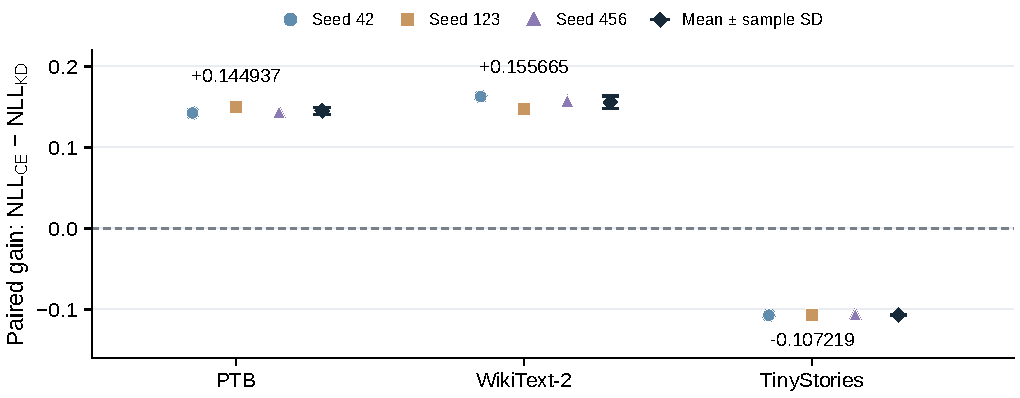
\includegraphics[width=\textwidth]{figures/fig2_cross_domain_gain.pdf}
\caption{CE-relative test-NLL transfer. Dots show independent student seeds; black markers and bars show the mean and sample SD. Positive values favor KD. Teachers and splits are fixed within each corpus.}
\label{fig:cross_domain_gain}
\end{figure*}

\section{What Determines Distillability?}\label{sec:distillability}

\subsection{Teacher-state reversal at fixed composition}
\label{sec:teacher-state}
At the same $\alpha=0.5$, jointly trained J has teacher validation-subset NLL 4.300644, compared with 6.376220 for fusion-weight-only A. J improves all three students by $+0.155665\pm0.007692$ NLL, whereas A harms all three with gain $-0.027654\pm0.006822$. The paired state contrast is
\begin{equation}
Q=\mathrm{NLL}_{\mathrm{KD,A}}-\mathrm{NLL}_{\mathrm{KD,J}},
\label{eq:teacher-state-contrast}
\end{equation}
averaging $+0.183319\pm0.001375$, positive in all three seeds.

Teacher training state and resulting predictive quality strongly modulate transfer at fixed architecture and composition. This is not scalar-likelihood causality: joint training also changes representations and errors, and teacher training budgets differ. Appendix~\ref{app:protocols} retains the original modes and eligibility amendments.

\subsection{A weaker source still transfers positively}
\label{sec:weaker-teacher}
The Grassmann-only source has validation-subset NLL 4.652064, worse than every matched validation-selected CE comparator on that subset. Nevertheless, all three students improve, with mean test gain $+0.040991\pm0.006733$. The comparator is the selected CE continuation, not an arbitrary initialization. Teacher likelihood is compared against the matched CE endpoint on the same validation subset, whereas transfer gain is evaluated on the selected test endpoints (Appendix~\ref{app:per-seed}).

Together, these controls show that teacher quality matters strongly but global held-out likelihood alone is insufficient to determine useful supervision. They neither make teacher quality irrelevant nor attribute positive transfer to geometry (Figure~\ref{fig:teacher_quality}).

\begin{figure*}[!t]
\centering
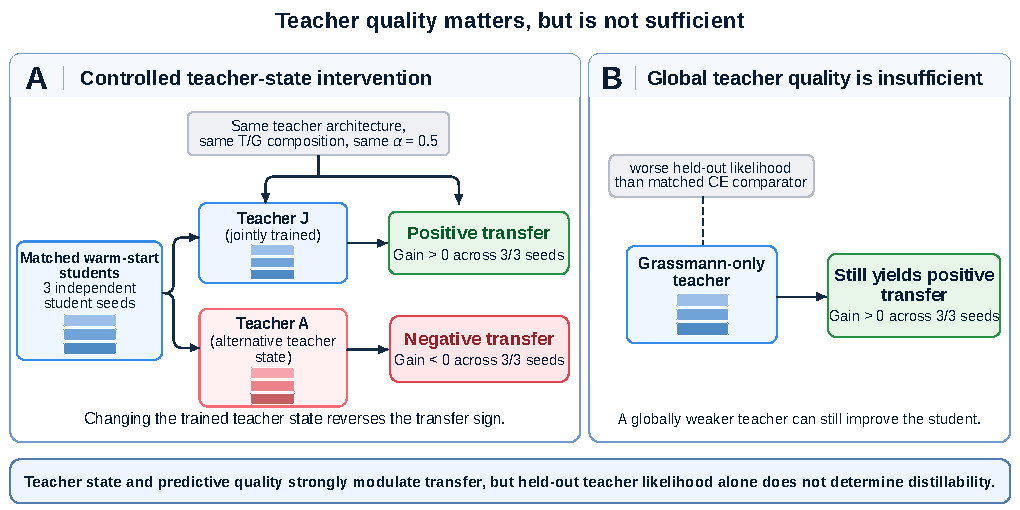
\includegraphics[width=\textwidth]{figures/fig3_teacher_quality.pdf}
\caption{WikiText-2 state and likelihood controls. Changing trained teacher state reverses transfer at fixed composition; a source with worse likelihood than CE still transfers positively. Neither establishes scalar-likelihood causality or a geometric KD advantage.}
\label{fig:teacher_quality}
\end{figure*}

\section{Source, Ensemble, and Diagnostic Controls}\label{sec:controls}

\subsection{Fused and component supervision}
\label{sec:source-ablation}
Holding J fixed, mean gains are $+0.155665$ for F, $+0.134868$ for T, and $+0.040991$ for G. F exceeds T by $+0.020797\pm0.001214$ and G by $+0.114674\pm0.001001$, with both contrasts positive in all three seeds. Composition and predictive quality change together, so this does not isolate the source of fusion benefits.

The T-only eligibility gate and first formal epoch clip every update despite finite parameter gradients. The authorized continuation retains \texttt{CLIP\_SATURATION\_WARNING}. Interpret the modest F--T gap cautiously; Appendix~\ref{app:protocols} records the unchanged training protocol and clipping trajectory.

\subsection{Homogeneous ensemble falsification}
\label{sec:homogeneous-control}
TT gives gain $+0.168125\pm0.008948$ versus $+0.155665\pm0.007692$ for TG. The paired contrast is
\begin{equation}
H=\mathrm{Gain}_{\mathrm{TG}}-\mathrm{Gain}_{\mathrm{TT}}
=\mathrm{NLL}_{\mathrm{TT}}-\mathrm{NLL}_{\mathrm{TG}},
\label{eq:ensemble-contrast}
\end{equation}
with mean $-0.012460\pm0.001348$ and all three differences negative. The tested TG teacher provides no advantage over TT (Figure~\ref{fig:ensemble_control}).

TT also has a 0.010108 full-validation teacher-NLL advantage, approximately 6.38\% fewer parameters, and different fusion-learning-rate and training histories. These confounds prevent attributing the ordering to intrinsic TT superiority. TG has greater branch disagreement, but not greater KD gain; predictive diversity is not necessarily transferable diversity. This comparison does not support a Grassmann-specific or heterogeneous-supervision advantage.

\subsection{Local diagnostics do not separate endpoints}
\label{sec:local-diagnostics}
Across seven teacher--domain families and three student seeds per family, retrospective first- and second-order scores both achieve AUROC approximately 0.644 and sign accuracy approximately 0.571. Curvature adds no sign separation, and the scores misclassify known positive WikiText-2 families. The tested local diagnostics are not reliable predictors of these endpoints.

Some scalar predictors discriminate pooled outcomes better, but the small dependent collection does not establish a general selection rule. Token-level branch JSD adds little information beyond CE difficulty. Appendix~\ref{app:diagnostics-modern} reports full metrics, calibration instability, and observational limits. The failures concern the tested offline scores, not adaptive KD methods in general.

\begin{figure*}[!t]
\centering
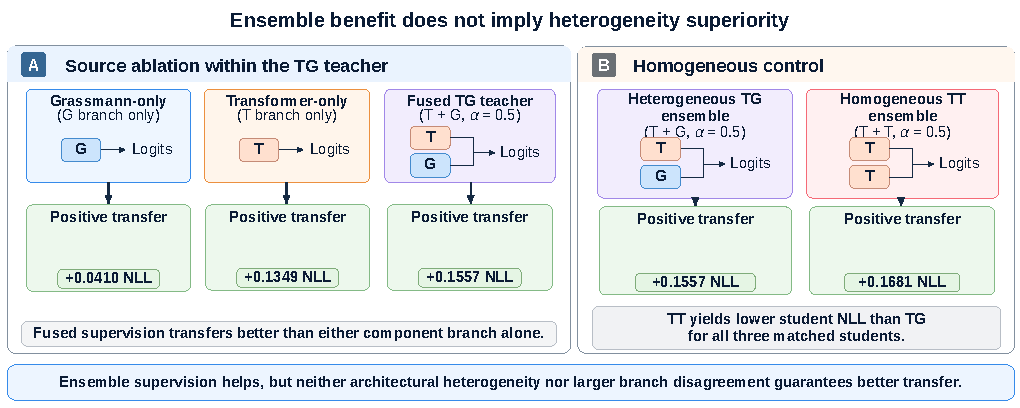
\includegraphics[width=\textwidth]{figures/fig4_ensemble_control.pdf}
\caption{WikiText-2 teacher-source and ensemble gains, rounded to four decimals. TT exceeds TG in all three students. T-only: early clipping saturation; interpret F--T gap cautiously. TT and TG teachers are not strictly quality- or training-matched.}
\label{fig:ensemble_control}
\end{figure*}

\section{External-Validity Stress Test}\label{sec:external-validity}

On a fixed FineWeb-Edu subset~\citep{penedo2024fineweb}, a frozen adapted SmolLM2-360M teacher supervises three independently adapted SmolLM2-135M students~\citep{benallal2025smollm2}. Gains are $-0.013550\pm0.003542$ at $\lambda=1$ and $-0.043924\pm0.004017$ at $\lambda=5$, both 3/3 negative with agreeing validation/test directions despite better teacher likelihood.

However, allowing $S_0$ as a step-0 validation candidate selects $S_0$ for all nine CE/KD continuations. This diagnostic does not replace primary trained-checkpoint endpoints; it shows that further CE itself is unnecessary in this regime. KD5 retains \texttt{CLIP\_SATURATION\_WARNING}; KD1 also clips frequently. Neither observation establishes clipping as the cause of degradation.

A CE-only headroom control uses a fixed early student and disjoint additional targets. Its best validation improvement, $+0.004849$, fails the preregistered 0.01 gate. Conditional KD and new test evaluation were therefore not performed. These results remain a bounded stress test, not clean modern-scale confirmation of harmful KD (Appendix~\ref{app:diagnostics-modern}).

\section{Discussion}\label{sec:discussion}

The evidence is consistent with configuration-dependent distillability, evaluated relative to a particular student state, CE comparator, and training protocol. Teacher quality strongly modulates transfer, yet a held-out average does not fully describe which predictive targets help a student. The state reversal and weaker-source counterexample can therefore coexist without identifying a complete causal decomposition.

Predictive diversity need not be transferable diversity: the more disagreeing TG teacher transfers less than TT in a confounded control. Similarly, local gradients summarize a small neighborhood, whereas full training changes parameters through scheduling and clipping regimes. These mismatches suggest caution in using the tested statistics as long-horizon predictors, not a universal impossibility of predicting KD. For a trained LM, matched CE continuation remains the relevant operational comparator.

The controls constrain distinct explanations rather than estimate interchangeable effects. The teacher-state comparison holds deployed architecture and composition fixed but changes branch states and preparation. The source ablation changes both composition and likelihood. The TT control tests whether a homogeneous alternative can match or exceed TG, not a parameter- and quality-matched architecture contrast. Shared CE and TG endpoints make the comparisons coherent within a student but do not multiply the independent evidence. Their joint interpretation is narrower than any isolated mechanism claim.

Checkpoint eligibility also changes the practical question. TinyStories CE improves from $S_0$, so its negative gain is relative to a useful continuation. In the modern stress test, allowing step 0 instead retains $S_0$ for every arm; poorer KD than CE coexists with little reason to continue either way. Reporting this distinction prevents treating all negative gains as evidence of the same training regime. None of these controls supports a universal rule for selecting teachers or tuning KD strength.

\section{Conclusion}\label{sec:conclusion}

Paired warm-start continuations show reproducible positive transfer on PTB and WikiText-2 and negative transfer on TinyStories. Changing trained teacher state reverses transfer at fixed composition, while a globally weaker source still improves all three students. Ensemble supervision is useful in the tested control, but TG has no advantage over TT. These bounded findings support configuration-dependent evaluation rather than a geometric mechanism or universal teacher-selection rule.
\label{end:main-text}

\section*{Limitations}\label{sec:limitations}

Primary students are small, and three student seeds give limited coverage of initialization variability. Corpora and teachers are fixed within each domain; student replications are not teacher replications. Controls share CE and TG endpoints and are not independent factorial experiments. No fully factorial intervention separates teacher quality, architecture, error structure, and optimization. The state intervention changes teacher training histories as well as predictive quality. TT/TG likelihood, parameter-count, and training mismatches prevent an isolated architecture comparison.

Clipping warnings and nonzero AMP skips limit optimization-based interpretation. T-only supervision clips every update early in training, and modern KD5 remains fully clip-saturated. No adaptive-KD baseline was evaluated; the study cannot establish superiority over adaptive methods. The local diagnostic collection is small, dependent, and retrospective rather than a prospective teacher-selection benchmark.

The modern stress test occurs in a degenerate continuation regime, and the CE-only headroom gate fails. SmolLM2 pretraining includes FineWeb-derived data, but exact document-level overlap with the selected subset remains unknown. Modern seeds independently adapt one pretrained student base rather than replicate pretraining. Generalization to larger students, other teachers, generative task metrics, and different continuation regimes remains unresolved.

% The official acl.sty already selects acl_natbib; do not select it twice.
\bibliography{references}
\clearpage
\appendix
\setcounter{figure}{0}
\renewcommand{\thefigure}{A\arabic{figure}}
\renewcommand{\theHfigure}{appendix.\arabic{figure}}
\section{Architecture and Experimental Details}\label{app:architecture}

The causal Grassmann branch uses local past--present pairs, not future-token pairs. A token embedding $h_t\in\mathbb R^d$ is reduced to $z_t=W_{\mathrm{red}}h_t+b_{\mathrm{red}}\in\mathbb R^r$. For $\mathcal D_t=\{\Delta\in\{1,2,4\}:t-\Delta\geq0\}$, the direction is $z_{t-\Delta}\rightarrow z_t$, and the exterior-product coordinates are
\begin{equation}
p_{ij,t}^{(\Delta)}=z_{t,i}z_{t-\Delta,j}-z_{t,j}z_{t-\Delta,i},\quad i<j.
\end{equation}
There are $r(r-1)/2$ coordinates. The subspace background follows basis equivalence on Grassmann manifolds~\citep{edelman1998geometry}. The exterior-product interpretation of Pl\"ucker coordinates is described in the geometric-algebra reference.\footnote{\url{https://cs.uwaterloo.ca/~smann/GA/plucker_coordinates.html}; background only, not evidence about KD.}
Dependent vectors have zero exterior product; normalization remains finite:
\begin{equation}
\widehat p_t^{(\Delta)}=\frac{p_t^{(\Delta)}}{\max(\|p_t^{(\Delta)}\|_2,\epsilon)},\quad\epsilon=10^{-8}.
\end{equation}
Geometric projection precedes the valid-window mean:
\begin{align}
g_t^{(\Delta)}&=W_{\mathrm{plu}}\widehat p_t^{(\Delta)}+b_{\mathrm{plu}},\\
g_t&=\frac{\sum_{\Delta\in\mathcal D_t}g_t^{(\Delta)}}{\max(1,|\mathcal D_t|)}.
\end{align}
An empty window gives zero. Mixing uses a feature-dependent vector gate:
\begin{align}
a_t&=\sigma(W_{\mathrm{gate}}[h_t;g_t]+b_{\mathrm{gate}}),\\
h_t^{\mathrm{mix}}&=a_t\odot h_t+(1-a_t)\odot g_t.
\end{align}
LayerNorm, dropout, and residual feed-forward processing surround this core. The LM head produces G logits independently of the Transformer logits; scalar $\alpha$ applies only at late fusion (Equation~\ref{eq:teacher-fusion}). Figure~\ref{fig:teacher_architecture} is generic and does not fix $\alpha=0.5$.

The compact primary student uses six layers, width 224, eight Transformer heads, reduced width 56, dropout 0.1, and final-block fusion. It has 31,434,257 parameters. The local GPT-2 tokenizer has vocabulary size 50,257 without added special tokens. Teacher dimensions and states follow their source configurations, not the student dimensions. The architecture is an existing test bed, not a geometry-specific method contribution.

\begin{figure*}[!t]
\centering
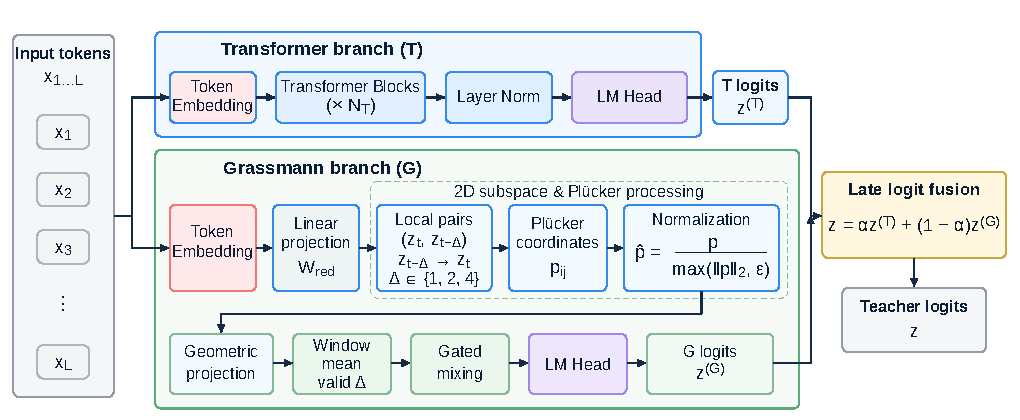
\includegraphics[width=\textwidth]{figures/figA1_teacher_architecture.pdf}
\caption{Generic heterogeneous teacher. The Grassmann path uses causal local pairs, normalized Pl\"ucker coordinates, geometric projection, valid-window averaging, gated mixing, and an LM head. Late fusion acts on logits with free $\alpha$. The architecture does not establish geometric KD superiority.}
\label{fig:teacher_architecture}
\end{figure*}

\section{Training Protocols and Important Amendments}\label{app:protocols}

\subsection{Corpora and matched students}
PTB and WikiText-2 use archived native splits; TinyStories uses a seed-42 98/2 train-derived split and the original validation split as test. PTB includes 42,068 nonempty training lines and 4,439 training chunks. TinyStories uses 300,000 training lines (67,081,279 pre-trim tokens; 262,036 chunks), 42,391 validation lines (9,440,302 tokens; 36,876 chunks), and 21,990 test lines (4,765,822 tokens; 18,616 chunks). Fixed 256-token chunks contribute positions 1--255 to evaluation; held-out targets do not enter training.

Each primary seed prepares its own $S_0$ using 20 epochs, batch 32, learning rate $2\times10^{-4}$, weight decay 0.01, AMP, and validation-NLL selection. Preparation uses AdamW with the source implementation defaults and a fixed learning rate. Continuations reset AdamW and use 10 epochs, batch 32, learning rate $10^{-4}$, weight decay 0.01, 5\% linear warmup followed by cosine decay, AMP, clipping at 1, and $\tau=2$. Only $\lambda$ differs between CE (0) and KD (5). Forward KL averages over valid target tokens, including temperature-squared scaling. Settings were frozen before these manuscript changes.

The common WikiText-2 subset comprises 512 validation chunks sampled without replacement using seed 20260920, then sorted (130,560 targets). Full-validation TT/TG metrics remain separate. Repeated J subset evaluations of 4.300644 and 4.300646 retain their original precision rather than being averaged together.

\subsection{Teacher preparation and eligibility}
Table~\ref{tab:teacher_training_protocol} records the teacher-training modes. J and TT have ten joint epochs; A has five fusion-weight-only epochs. The state intervention fixes deployed architecture and composition, not teacher training history. TT source Transformers have six layers, width 256, dropout 0.1, batch 32, learning rate $3\times10^{-4}$, and 20 preparation epochs, with seeds 42 and 123; both select epoch 12. TT joint training selects epoch 10. Its fusion learning rate differs from historical TG.
\begin{table*}[!t]\centering
\begin{tabular}{llrrr}
\toprule
Teacher & Mode & Epoch budget & Branch LR & Fusion-weight LR\\
\midrule
J/TG & Joint & 10 & $10^{-5}$ & $5\times10^{-3}$\\
A & Fusion weight only & 5 & Frozen & $10^{-2}$\\
TT & Joint & 10 & $10^{-5}$ & $10^{-2}$\\
\bottomrule
\end{tabular}
\caption{Archived WikiText-2 teacher-training configurations. All initialize $\alpha=0.5$, use batch 32, weight decay 0.01 and AMP, and select by validation. Joint arms freeze branches in epoch 1; A freezes them throughout. Evaluation and KD force $\alpha=0.5$. These histories do not isolate scalar teacher quality or architecture.}
\label{tab:teacher_training_protocol}
\end{table*}


Joint training changes 179 of 191 J/A state tensors. A reduced-data eligibility smoke had clip fraction 1 and AMP/nonfinite fraction 0.16. An authorized full-data one-epoch gate replaced it without changing the objective or clip threshold. J/A gate clip fractions were 0.234694 and 0.275510, both with AMP/nonfinite fraction 0.013605. A/J parameter-gradient ratios of 1.102792, 1.148522, and 1.093056 satisfy the registered interval $[0.5,2]$. Formal A first-epoch clip fractions were 0.666667, 0.503401, and 0.513605; maximum AMP/nonfinite fraction was 0.013605.

T-only required a separate authorized eligibility amendment: the full-data gate clipped every update but retained finite parameter gradients, T/F ratios 1.3164, 1.2788, and 1.2324, and AMP/nonfinite fraction 0.013605. Formal training retained all settings. First epochs remained fully saturated; mean epoch clip fractions were 0.4990, 0.4605, and 0.4398, falling to approximately 0.0034 late in training. All select epoch 10. The permanent \texttt{CLIP\_SATURATION\_WARNING} limits interpretation of the F--T gap.

TT student first-epoch clip fractions were 0.928571, 0.843537, and 0.874150; corresponding means over epochs were 0.170068, 0.137755, and 0.127551. Maximum AMP/nonfinite fraction was 0.013605. These trajectories are not strict optimization matches to TG.

\subsection{TinyStories stability and accepted retry}
All primary TinyStories CE and KD arms select epoch 10. CE mean clipping is 0.000391 in each seed; KD means are 0.236891, 0.283344, and 0.240090 (Table~\ref{tab:tinystories_optimization}). Maximum AMP/nonfinite fractions are 0.000488 for CE and 0.000611 for KD. Accepted endpoints are finite, and KD is not persistently fully clip-saturated.

One seed-456 attempt was interrupted in epoch 2 because of an infrastructure power cap and excluded before any final endpoint existed. The authorized completed retry restarted from identical $S_0$ with a fresh optimizer and unchanged teacher, seed, data, objective, budget, and selection. Only the completed retry contributes to results. Experiments used RTX 3090 GPUs; detailed aggregate compute accounting is unavailable and is not inferred here.
\begin{table*}[!t]\centering
\begin{tabular}{lrrrrr}
\toprule
Seed & Residual & KD KL & CE norm & KD norm & KD clip \\
\midrule
42 & -0.021960 & 0.380224 & 0.486891 & 0.973546 & 0.236891 \\
123 & -0.021422 & 0.381402 & 0.488263 & 0.981438 & 0.283344 \\
456 & -0.019714 & 0.383282 & 0.483211 & 0.973942 & 0.240090 \\
\bottomrule
\end{tabular}
\caption{Primary TinyStories telemetry. Residual is teacher advantage over the CE test endpoint. KL includes temperature-squared scaling; norms and clip fractions are epoch means across the completed run.}\label{tab:tinystories_optimization}
\end{table*}


\section{Full Per-Seed Results}\label{app:per-seed}

Table~\ref{tab:per_seed_gains} gives paired test gains for the confirmatory families. Gains derive from archived NLL, not logarithms of rounded PPL. All WikiText-2 arms within a seed share its CE comparator, and J/TG is one reused endpoint. Mean CE/KD test NLLs are 4.082352/3.937415 for PTB, 4.276364/4.120699 for WikiText-2, and 1.582197/1.689416 for TinyStories. Tables~\ref{tab:ptb_endpoints}, \ref{tab:wt2_endpoints}, and~\ref{tab:ts_endpoints} report selected endpoints.
\begin{table*}[!t]\centering
\begin{tabular}{lrrr}
\toprule
Condition & Seed 42 & Seed 123 & Seed 456 \\
\midrule
PTB fused & 0.142284 & 0.149462 & 0.143066 \\
TinyStories fused & -0.107479 & -0.107439 & -0.106740 \\
WT2 J/TG & 0.162501 & 0.147337 & 0.157157 \\
WT2 A & -0.022394 & -0.035362 & -0.025206 \\
WT2 G & 0.046771 & 0.033598 & 0.042604 \\
WT2 T & 0.142785 & 0.125226 & 0.136593 \\
WT2 TT & 0.176453 & 0.158666 & 0.169257 \\
\bottomrule
\end{tabular}
\caption{Archived paired test-NLL gains. Positive values favor KD; every WikiText-2 arm shares the same CE endpoint within a seed.}\label{tab:per_seed_gains}
\end{table*}

\begin{table*}[!t]\centering
\begin{tabular}{lrrrrrr}
\toprule
Seed & CE test & KD test & CE val. & KD val. & CE epoch & KD epoch \\
\midrule
42 & 4.079528 & 3.937244 & 4.237272 & 4.081793 & 1 & 10 \\
123 & 4.088605 & 3.939143 & 4.243102 & 4.082198 & 1 & 10 \\
456 & 4.078925 & 3.935859 & 4.244354 & 4.082000 & 1 & 9 \\
\bottomrule
\end{tabular}
\caption{PTB test and validation NLL from the archived selected-checkpoint summaries. The paired differences match the confirmatory inventory; epochs are independently validation-selected.}\label{tab:ptb_endpoints}
\end{table*}

\begin{table*}[!t]\centering
\begin{tabular}{lrrrrrr}
\toprule
Seed & CE & KD(J/TG) & KD(T) & KD(G) & KD(A) & KD(TT) \\
\midrule
42 & 4.270742 & 4.108241 & 4.127957 & 4.223972 & 4.293136 & 4.094289 \\
123 & 4.277520 & 4.130183 & 4.152294 & 4.243922 & 4.312882 & 4.118854 \\
456 & 4.280830 & 4.123673 & 4.144237 & 4.238226 & 4.306036 & 4.111574 \\
\bottomrule
\end{tabular}
\caption{WikiText-2 selected student test NLL. J/TG is the same reused fused endpoint, not two experiments. All KD columns report student endpoints, not teacher likelihood.}\label{tab:wt2_endpoints}
\end{table*}

\begin{table*}[!t]
\centering
\begin{tabular}{lrrrr}
\toprule
Seed & $S_0$ test & CE test & KD test & KD--CE validation\\
\midrule
42 & 1.622437 & 1.581269 & 1.688747 & 0.108394\\
123 & 1.623954 & 1.581807 & 1.689246 & 0.108082\\
456 & 1.624901 & 1.583515 & 1.690255 & 0.108040\\
\bottomrule
\end{tabular}
\caption{TinyStories selected NLLs. All arms select epoch 10. Positive validation KD--CE differences agree with negative CE-relative test gains.}
\label{tab:ts_endpoints}
\end{table*}


The G teacher residual advantages over the validation-selected CE endpoints on the common subset are $-0.266520$, $-0.253492$, and $-0.251006$, while test gains are $+0.046771$, $+0.033598$, and $+0.042604$. The reference is CE, not $S_0$. Teacher likelihood and gains have different held-out scopes; these seeds do not independently replicate teacher training.

Teacher-state contrast $Q$ is 0.184895, 0.182699, and 0.182364 for seeds 42, 123, and 456, averaging $0.183319\pm0.001375$. Source means and sample SDs are F $0.155665\pm0.007692$, T $0.134868\pm0.008906$, and G $0.040991\pm0.006733$. F--T and F--G differences are $0.020797\pm0.001214$ and $0.114674\pm0.001001$, respectively. Teacher-source subset NLLs are 4.300646, 4.445647, and 4.652064. Composition changes also change quality.

On full validation, TG/TT teacher NLLs are 4.303697/4.293589; branch NLLs are 4.451680/4.655020 for TG and 4.406160/4.422151 for TT. TG has 37,749,633 parameters, TT 35,340,801. Their KD gains are $0.155665\pm0.007692$ and $0.168125\pm0.008948$. The paired $H$ mean is $-0.012460\pm0.001348$, all three negative. Table~\ref{tab:branch_comparison} keeps full-validation branch metrics separate from the subset intervention. Higher TG disagreement does not yield better transfer, but quality, count, and history confounds prevent a causal architecture or diversity comparison.
\begin{table*}[!t]
\centering
\begin{tabular}{lrrrr}
\toprule
Teacher & Full-validation NLL & Branch JSD & Agreement & Fusion gain\\
\midrule
TG & 4.303697 & 0.182087 & 0.507034 & 0.147983\\
TT & 4.293589 & 0.099793 & 0.630170 & 0.112570\\
\bottomrule
\end{tabular}
\caption{Full-validation teacher comparison at $\alpha=0.5$. Fusion gain is NLL improvement over the better branch. Quality, parameter counts, and training histories differ. These metrics are not pooled with the 512-chunk state/source subset.}
\label{tab:branch_comparison}
\end{table*}


\section{Diagnostic and Modern Stress-Test Details}\label{app:diagnostics-modern}

\subsection{Branch disagreement and retrospective probes}
On the common validation subset, J branch NLLs are 4.445648 and 4.652064, JSD 0.181288, agreement 0.508395, and fusion gain 0.145003 over the better branch. A has branch NLLs 6.540640 and 6.696787, JSD 0.176641, agreement 0.543719, and fusion gain 0.164420. Quality changes substantially, without a uniformly favorable shift in disagreement or fusion gain.

Token-level disagreement analysis uses one selected CE/KD pair per corpus, not three model replications. Adding JSD beyond CE token difficulty gives incremental gradient-conflict AUROC $-0.000323$ on PTB and $+0.010910$ on TinyStories; incremental endpoint $R^2$ is $+0.000533$ and $+0.003061$. Token/chunk bootstrap uncertainty does not create independent model seeds. These small increments do not establish disagreement as a strong transfer mechanism.

Local diagnostics span seven families and 21 dependent seed-level conditions. Training probes use the first 32 chunks, with FP32 microbatches of two over all student parameters. Calibration seeds 314159, 271828, and 161803 each select two disjoint validation chunks, giving 63 rows. Scores were frozen before endpoint merging; no test data entered probes and no updates were retained.

At $S_0$, let $g=\nabla\mathcal L_{\mathrm{CE}}$, $k=\nabla\mathcal L_{\mathrm{distill}}$, $v=\nabla\mathcal L_{\mathrm{val}}$, and $H_{\mathrm{val}}=\nabla^2\mathcal L_{\mathrm{val}}$. Define $a=v^\top k$, $b=g^\top H_{\mathrm{val}}k$, and $c=k^\top H_{\mathrm{val}}k$. The nominal Taylor diagnostic is
\begin{equation}
\widehat G_{\mathrm{local}}(\lambda)=\eta\lambda a-\eta^2\lambda b-\tfrac12\eta^2\lambda^2c,
\end{equation}
with $\eta=10^{-4}$. It is not a bound on the selected test endpoint. All gradients and HVPs are finite; first-/second-order signs agree in 63/63 rows, with seed-level AUROC 0.644444, sign accuracy 0.571429, and family-mean AUROC 0.600000. Both miss positive WikiText-2 J, G, and TT families. Only 11/21 conditions have stable signs across calibration subsets. Median absolute curvature correction is $2.73\times10^{-7}$ (0.52\% of the first-order magnitude) and never changes a sign.

The literal first scheduled step has zero learning rate and is a no-op, not a safety result. A nominal-rate clipped AdamW virtual diagnostic has AUROC 0.700000 and accuracy 0.571429; it misses 9/15 beneficial outcomes and has stable signs in 10/21 conditions. Table~\ref{tab:full_predictors} reports pooled retrospective scores. Dependence and small coverage preclude a universal selection rule or an adaptive-method comparison.
\begin{table*}[!t]\centering
\begin{tabular}{lrrr}
\toprule
Predictor & AUROC & Sign accuracy & $\rho$ \\
\midrule
Teacher residual & 0.711111 & 0.523810 & 0.437662 \\
Teacher val NLL & 0.500000 & -- & 0.235921 \\
KL magnitude & 0.722222 & -- & 0.450649 \\
KD grad norm & 0.500000 & -- & -0.118182 \\
Train CE-KD cosine & 0.477778 & 0.714286 & -0.024675 \\
Validation dot a & 0.644444 & 0.571429 & 0.249351 \\
Validation cosine & 0.644444 & 0.571429 & 0.285714 \\
Quadratic gain & 0.644444 & 0.571429 & 0.249351 \\
Virtual nominal gain & 0.700000 & 0.571429 & 0.427273 \\
\bottomrule
\end{tabular}
\caption{Full seed-level retrospective predictor comparison over 21 dependent conditions. A dash denotes a metric not defined for that predictor; it does not indicate zero.}\label{tab:full_predictors}
\end{table*}


\subsection{Modern continuation and checkpoint eligibility}
SmolLM2 base student/teacher models have 134,515,008/361,821,120 parameters and shared vocabulary 49,152. The 360M teacher is adapted once, then frozen. Student seeds independently adapt one pretrained 135M base, not independently pretrained models. FP32 weights use BF16 autocast and FP32 losses without GradScaler. AdamW uses learning rate $5\times10^{-5}$, weight decay 0.01, betas $(0.9,0.95)$, epsilon $10^{-8}$, 5\% warmup, and cosine decay. Sequence length is 256, batch 32, microbatch 4, clip threshold 1, and $\tau=2$. Each teacher adaptation, student preparation, and continuation receives 10M targets (1,221 updates).

FineWeb-Edu uses the first shard of the pinned \texttt{sample-10BT} revision. Deterministic document-ID hashing and exact-text deduplication produce disjoint training, validation, and test splits with 20M, 1M, and 1M encoded tokens; held-out splits evaluate 999,999 targets each. Primary validation candidates are steps 256, 512, 768, 1024, and 1221, excluding $S_0$. Test follows selection. Table~\ref{tab:modern_endpoints} reports those endpoints; Table~\ref{tab:modern_optimization} gives the selected steps and recorded telemetry.

Teacher validation/test NLLs are 2.747486/2.726017, better than every $S_0$. CE test NLL nevertheless increases from $S_0$ by 0.005562, 0.005268, and 0.012924 (mean $+0.007918\pm0.004338$). Allowing step 0 selects $S_0$ in all nine CE/KD arms and yields diagnostic CE-relative gain zero. This does not replace the trained-checkpoint primary comparison. Exact pretraining overlap remains unknown.
\begin{table*}[!t]\centering
\begin{tabular}{lrrrrr}
\toprule
Seed & Split & $S_0$ & CE & KD1 & KD5 \\
\midrule
42 & validation & 2.967112 & 2.973155 & 2.988861 & 3.019882 \\
42 & test & 2.944338 & 2.949900 & 2.965619 & 2.996304 \\
123 & validation & 2.967390 & 2.973067 & 2.988537 & 3.019533 \\
123 & test & 2.944865 & 2.950133 & 2.965603 & 2.996212 \\
456 & validation & 2.967554 & 2.980508 & 2.990422 & 3.020545 \\
456 & test & 2.944959 & 2.957883 & 2.967346 & 2.997173 \\
\bottomrule
\end{tabular}
\caption{Frozen FineWeb-Edu primary endpoints. Validation selection excludes step 0 for CE/KD. Test is evaluated only after that selection; the separate best-including-S0 diagnostic selects S0 in all nine arms.}\label{tab:modern_endpoints}
\end{table*}

\begin{table*}[!t]\centering
\begin{tabular}{lrrrrr}
\toprule
Seed & Arm & Step & Clip fraction & Mean norm & Max norm \\
\midrule
42 & S0 & 256 & 0.129402 & 0.947446 & 3.142341 \\
42 & CE & 1221 & 0.058968 & 0.929848 & 1.394476 \\
42 & KD1 & 1221 & 0.850123 & 1.084600 & 2.502529 \\
42 & KD5 & 1221 & 1.000000 & 2.557157 & 11.615945 \\
123 & S0 & 256 & 0.117117 & 0.948927 & 4.028796 \\
123 & CE & 1221 & 0.056511 & 0.929663 & 1.203820 \\
123 & KD1 & 1221 & 0.854218 & 1.090724 & 3.144516 \\
123 & KD5 & 1221 & 1.000000 & 2.601404 & 19.092007 \\
456 & S0 & 1221 & 0.127764 & 0.944769 & 1.363758 \\
456 & CE & 256 & 0.045045 & 0.994147 & 86.482155 \\
456 & KD1 & 1221 & 0.798526 & 1.074831 & 2.708021 \\
456 & KD5 & 1221 & 1.000000 & 2.545350 & 12.600890 \\
\bottomrule
\end{tabular}
\caption{FineWeb-Edu optimization audit. Step is selected by validation among trained checkpoints. Norms are measured before clipping; all recorded nonfinite and overflow fractions are zero.}\label{tab:modern_optimization}
\end{table*}


Initial unweighted KD/CE gradient ratios are 2.150561, 2.485828, and 2.462981. KD1 clip fractions are 0.850123, 0.854218, and 0.798526; KD5 clips every update. All recorded overflow/nonfinite fractions are zero. KD5 retains \texttt{CLIP\_SATURATION\_WARNING}. The seed-456 CE preclip norm reaches 86.482155 at step 711, after its selected step 256. Its cause and trajectory impact are unknown; the run remains included with \texttt{CE456\_GRADIENT\_SPIKE\_WARNING}.

\subsection{Failed disjoint-continuation headroom gate}
The CE-only control fixes the seed-42 preparation checkpoint at step 256, after 2,097,152 targets, rather than selecting $S_0$ by validation. Its frozen manifest excludes 8,192 consumed target chunks and supplies 31,250 new chunks (8M targets). Boundary context may be shared, but prediction targets are excluded. The manifest and order were fixed before continuation endpoints were observed.

Candidates $5\times10^{-6}$, $10^{-5}$, and $2\times10^{-5}$ retain the optimizer family, scheduler, batch, sequence length, clipping, and budget. Validation selection includes steps 0, 256, 512, 768, and 977, with earlier-checkpoint tie breaking. All select step 977. Improvements are 0.004214, 0.004849, and 0.003941, below the 0.01 gate (Table~\ref{tab:modern_ce_gate}); clip fractions are 0.060389, 0.079836, and 0.082907 with zero nonfinite fraction. The highest-rate arm has a finite norm spike 14.602655 at step 656 of unknown cause and impact.

The frozen decision is
\texttt{STOP\_MODERN\_CONTINUATION\_}\allowbreak\texttt{NOT\_ESTABLISHED}.
Conditional KD at $\lambda=0.25$ or 1, new test endpoints, and initial KD/CE gradient ratios were not measured. They are missing by design, not zero. The stress test does not establish that FineWeb-Edu causes negative transfer, better teachers generally harm KD, or all modern-model KD fails.
\begin{table*}[!t]
\centering
\begin{tabular}{lrrrr}
\toprule
CE peak LR & Selected val NLL & Val improvement & Selected step & Gate \\
\midrule
5e-06 & 2.962897 & 0.004214 & 977 & FAIL \\
1e-05 & 2.962263 & 0.004849 & 977 & FAIL \\
2e-05 & 2.963171 & 0.003941 & 977 & FAIL \\
\bottomrule
\end{tabular}
\caption{CE-only disjoint-continuation gate from fixed early $S_0$, seed 42. Validation selection includes step 0. No learning-rate candidate reaches the required 0.01 improvement, so conditional KD and new test evaluation are not performed.}
\label{tab:modern_ce_gate}
\end{table*}


\end{document}
